\documentclass[12pt]{article}
\usepackage[spanish]{babel}
\usepackage{makeidx}
\usepackage[margin=1in]{geometry}  % set the margins to 1in on all sides
\usepackage{graphicx}              % to include figures
\usepackage{amsmath}               % great math stuff
\usepackage{amsfonts}              % for blackboard bold, etc
\usepackage{amsthm}                % better theorem environments
\usepackage{makeidx}               % index
\usepackage[utf8]{inputenc}        % now we have tildes!
\usepackage{wrapfig}               % images
\usepackage{listings}              % Unordered lists
\usepackage{hyperref}              % hyperlinks
\usepackage{xcolor}                % to colorize font
\usepackage{blindtext}             % to colorize font
\usepackage{caption}
\usepackage{subcaption}

\makeindex

\begin{document}

\begin{titlepage}

\newcommand{\HRule}{\rule{\linewidth}{0.5mm}} % Defines a new command for the horizontal lines, change thickness here

\center % Center everything on the page

%----------------------------------------------------------------------------------------
%	LOGO SECTION
%----------------------------------------------------------------------------------------

\textsc{\LARGE Universidad Carlos III de Madrid}\\[1.2cm] % Name of your university/college

%----------------------------------------------------------------------------------------
%	HEADING SECTIONS
%----------------------------------------------------------------------------------------


\includegraphics[width=9cm]{Logo}\\[1.2cm] % Include a department/university logo - this will require the graphicx package

\textsc{\Large Aprendizaje Automático}\\[0.5cm] % Major heading such as course name
\textsc{\large Grado en Ingeniería Informática}\\[0.6cm] % Minor heading such as course title
\textsc{\large Grupo 83}\\[0.5cm]

%----------------------------------------------------------------------------------------
%	TITLE SECTION
%----------------------------------------------------------------------------------------

\HRule \\[0.7cm]
{ \huge \bfseries Tutorial 4: Introduccíon al aprendizaje por refuerzo}\\[0.4cm] % Title of your document
\HRule \\[0.7cm]

%----------------------------------------------------------------------------------------
%	AUTHOR SECTION
%----------------------------------------------------------------------------------------

\textit{Autores:}\\
Daniel \textsc{Medina García}\\ % Your name
Alejandro \textsc{Rodríguez Salamanca}\\[1.1cm] % Your name

%----------------------------------------------------------------------------------------
%	DATE SECTION
%----------------------------------------------------------------------------------------

{\large \today}\\ % Date, change the \today to a set date if you want to be precise

%----------------------------------------------------------------------------------------

\vfill % Fill the rest of the page with whitespace

\end{titlepage}

\tableofcontents

\newpage
\thispagestyle{empty}
\clearpage
\vspace*{\fill}
\begin{center}
    \begin{minipage}{\textwidth}
        \begin{center}
            \section*{Introducción}
            % TODO: Needed?
        \end{center}
    \end{minipage}
\end{center}
\vfill

\newpage
\section{Ejercicio 1}

En este primer ejercicio tomamos contacto con el programa ejecutando tanto el agente manual como el estándar.
Por cada movimiento ejecutado, en la salida por consola aparecen el estado inicial, la acción tomada, el estado al que se llega y la recompensa obtenida. El agente por defecto es \textit{random}, que toma acciones aleatorias entre las permitidas. La Figura 1 muestra los MDP deterministas requeridos en el enunciado del tutorial:

\begin{figure}[h]
    \centering
    \begin{subfigure}{.5\textwidth}
        \centering
        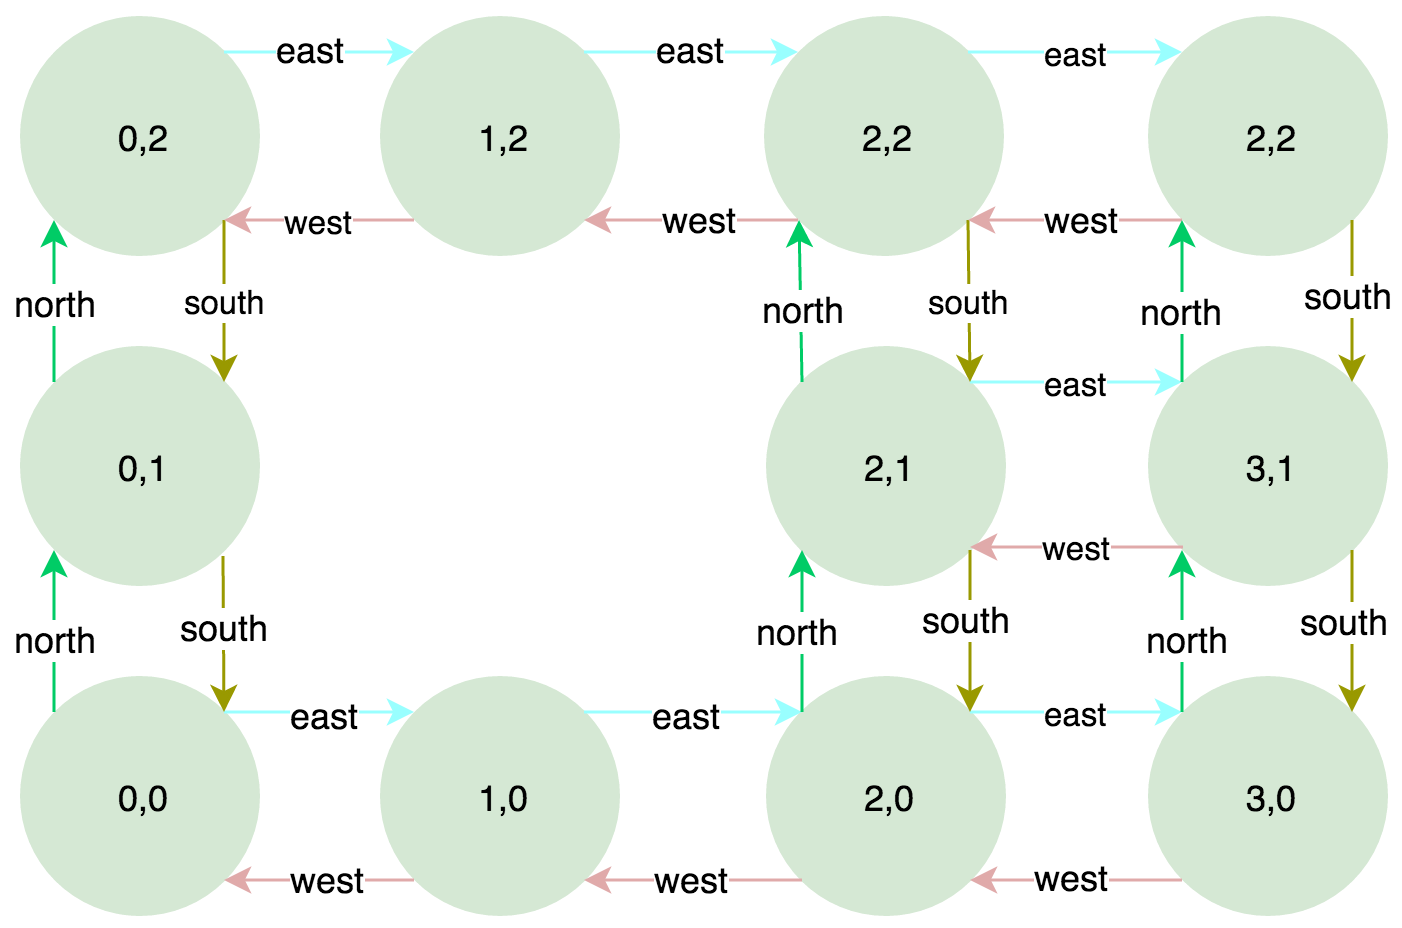
\includegraphics[width=.85\linewidth]{MDP_deterministic}
        \caption{Default grid}
        \label{fig:sub1}
    \end{subfigure}%
    \begin{subfigure}{.5\textwidth}
        \centering
        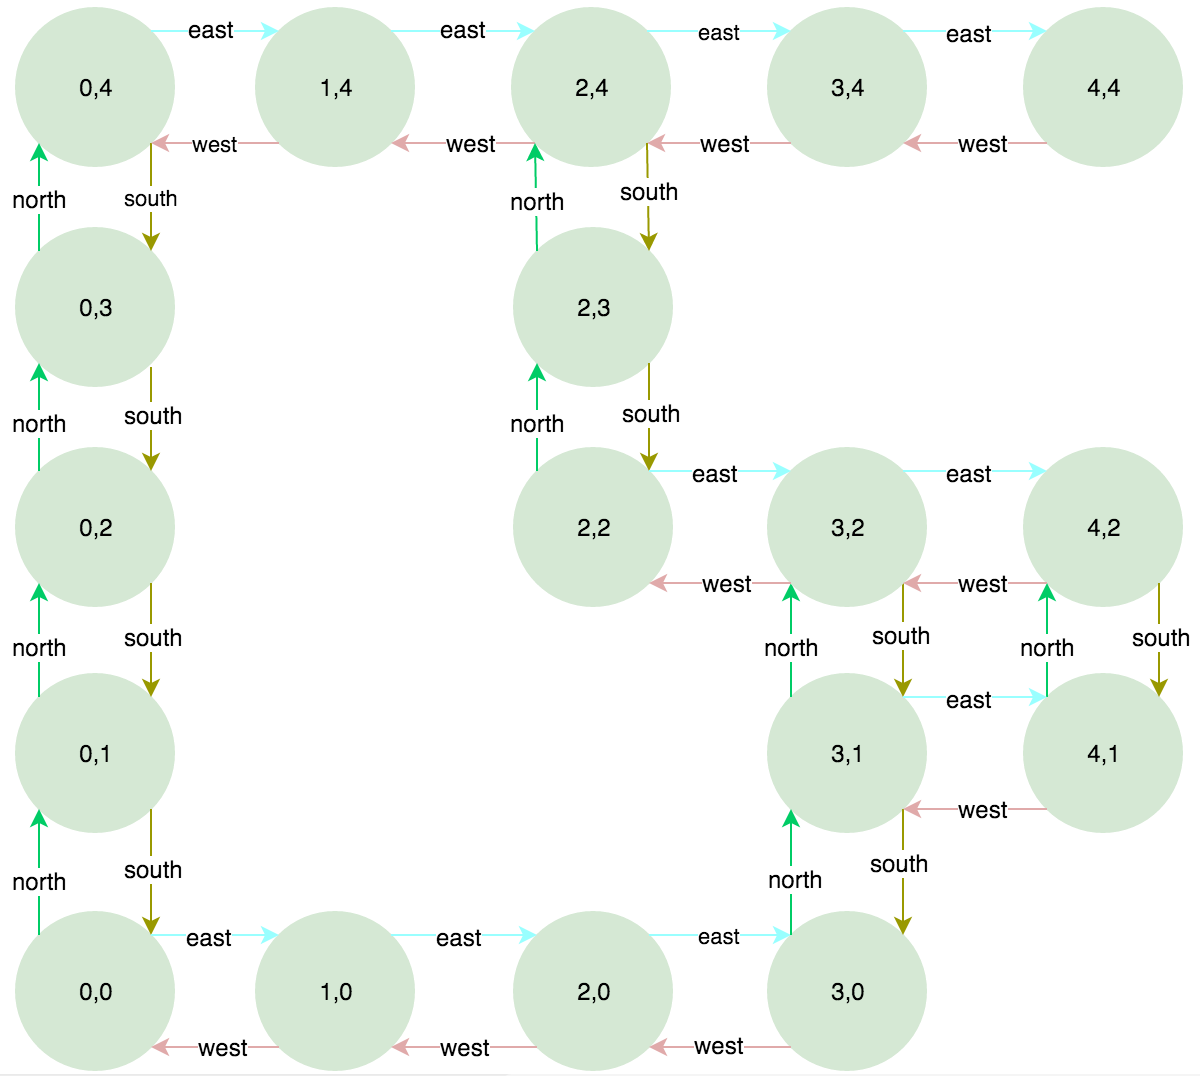
\includegraphics[width=.85\linewidth]{MDP_deterministic2}
        \caption{AAGrid}
        \label{fig:sub2}
    \end{subfigure}
    \caption{Deterministic MDPs}
    \label{fig:test}
\end{figure}

Estos laberintos, al igual que los demás incluidos en el código proporcionado, se almacenan en forma de arrays bidimensionales. Cada posición de la matriz representa una posición del laberinto, con los siguientes símbolos:
\begin{itemize}
    \item \textbf{Un espacio} representa una casilla común, sin recomensa ni coste algunos, por la que el agente puede pasar.
    \item \textbf{Un valor numérico} representa una casilla con una recompensa o un precio. Si el agente se mueve a esta casilla cambiará su puntuación añadiéndole el valor contenido en dicha casilla.
    \item \textbf{Una almohadilla (\#)} es considerada un muro, o casilla inalcanzable por el agente. Ninguna acción legal puede llevar al agente a estas posiciones.
    \item Por último, la posición de la que parte el agente se guarda como \textbf{una `S'}.
\end{itemize}

\newpage
\begin{wrapfigure}{r}{0.52\textwidth}
    \begin{verbatim}
          [[' ',' ',' ',' ',]
           ['8','#','3',' ',]
           ['#',' ',' ','#',]
           [' ',' ',' ',' ',]
           [' ','S','#',' ',]]
    \end{verbatim}
    \vspace{-20pt}
    \caption{New grid}
    \vspace{-10pt}
\end{wrapfigure}
De esta forma, podemos crear un nuevo laberinto siguiendo las instrucciones mencionadas. La siguiente figura muestra un laberinto creado por nosotros, en la que el agente deberá buscar una ruta sorteando los muros si quiere conseguir la mayor recompensa:\\[1em]

\huge Aquí contamos cómo cojones se pueden sacar varias políticas óptimas, describiendo todas las políticas óptimas para este problema. \small
https://webdocs.cs.ualberta.ca/~sutton/book/ebook/node41.html
\newpage
\section{Ejercicio 2}
https://webdocs.cs.ualberta.ca/~sutton/book/ebook/node65.html
\section{Ejercicio 3}


\end{document}
